\section{Nix/NixOS}

\begin{figureBox}[label={fig:nix-snowflake}]{the NixOS logo, also know as the Nix Snowflake.}
  
\includegraphics[width=0.2\linewidth]{./background/figures/nix/nix-snowflake.pdf}
\end{figureBox}

\textbf{Nix} \cite{dolstra2004nix} is an open-source, "purely functional package manager” used in unix-like operating systems to provide a functional and reproducible approach to package management. Started in 2003 as research project Nix \cite{dolstra2006purely} is widely used in both industry \cite{NixCommunityNixOSWiki} and academia \cite{10.1145/3152493.3152556} \cite{https://doi.org/10.1002/qua.26872} \cite{LHCbNix}, and its associated public package repository \texttt{nixpkgs} \cite{NixPkgs} as of Jan 2024 has over 80,000 unique packages making it the largest up-to-date package repository in the world as can be seen in Fig~\ref{fig:package-manager-comparison}. Out of Nix has also grown \textbf{NixOS} \cite{10.1145/1411204.1411255} \label{nix-snowflake} a Linux distribution that is conceived and defined as a deterministic and reproducible entity that is declared functionally and is built using the \textbf{Nix} package manager. \\

%% Repology Package Manager Comparison
\begin{figureBox}[label = {fig:package-manager-comparison}]{Comparison of all package repositories from Repology.org \cite{Marakasov_2024}}
  \fontsize{5}{6}\selectfont
  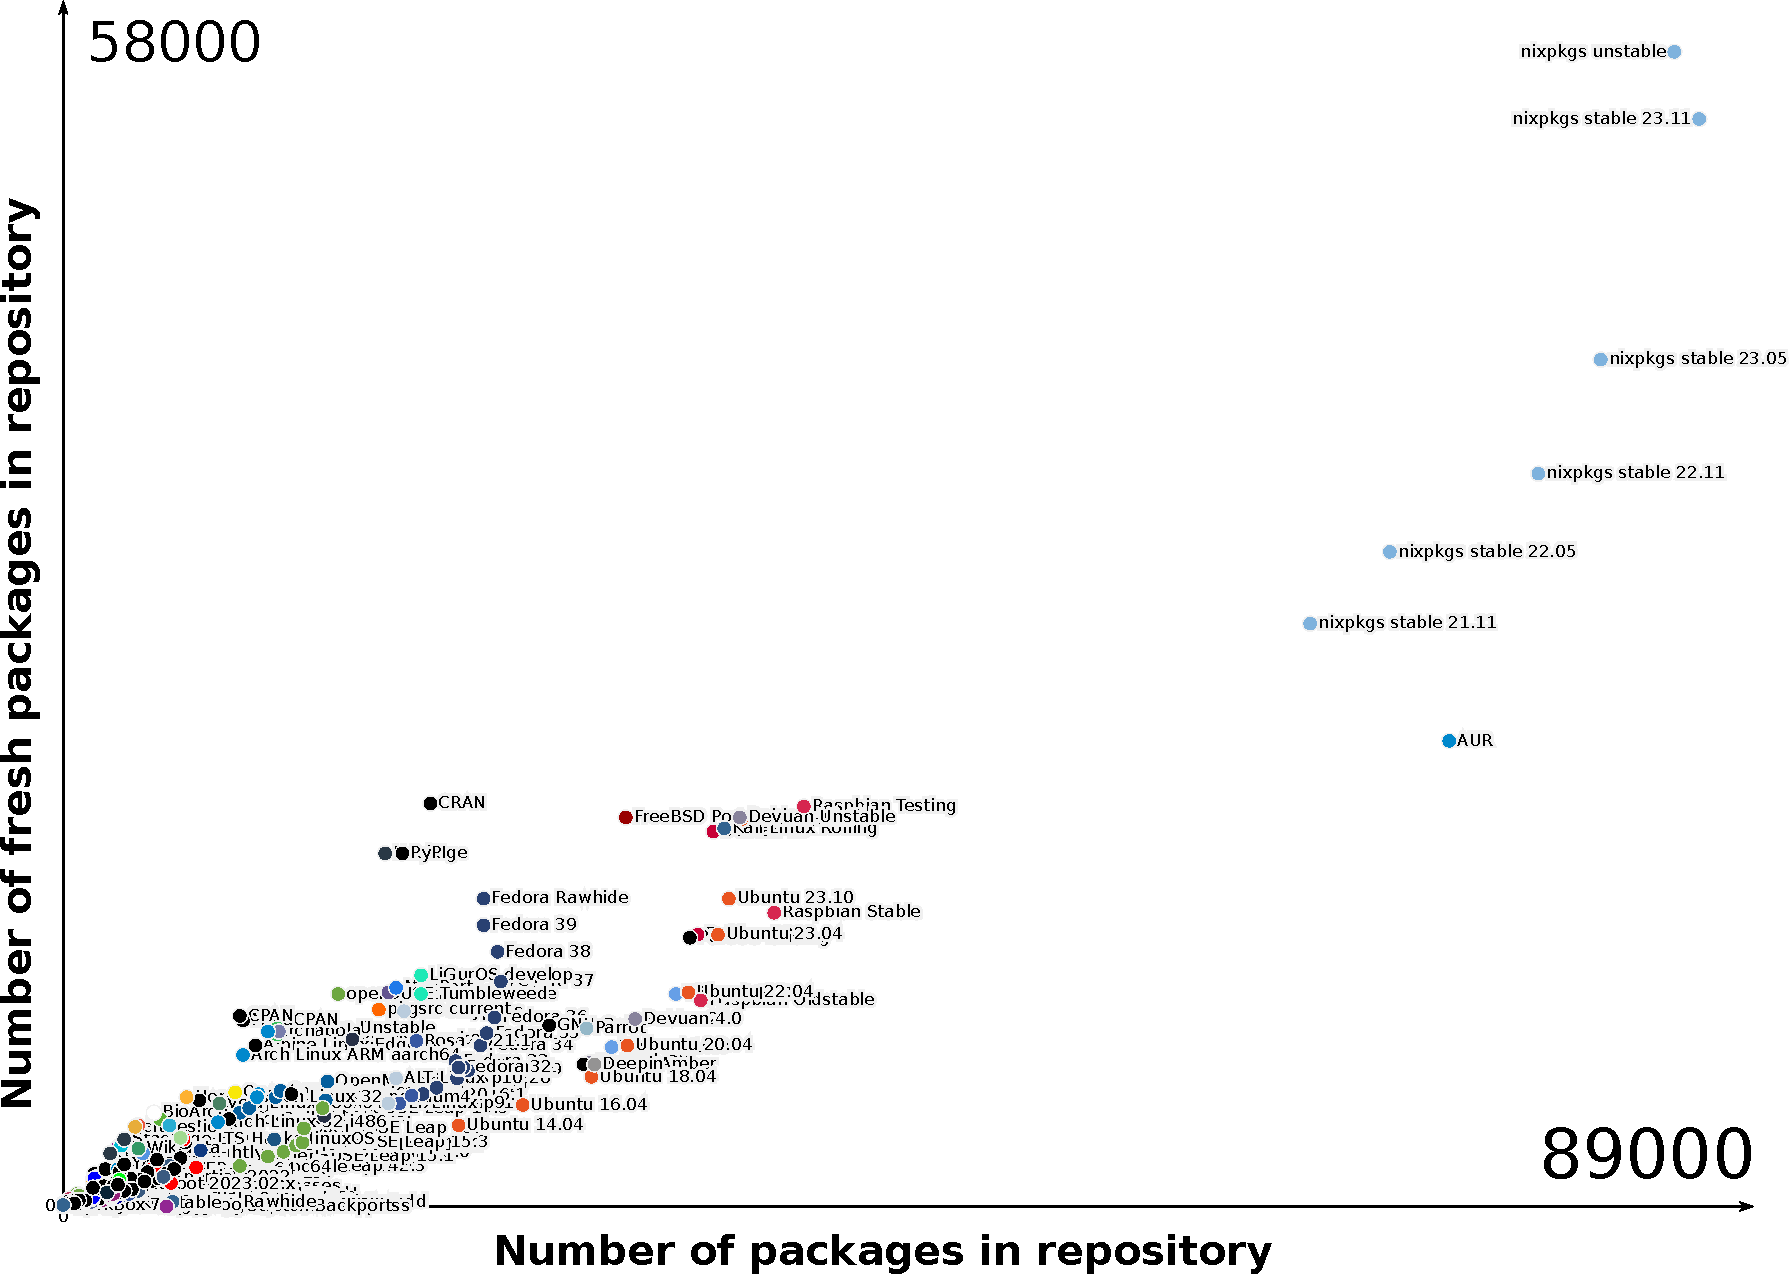
\includegraphics[width=\linewidth]{./background/figures/nix/pkg-compare.pdf}
\end{figureBox}

Nix packages are defined in the \textbf{Nix Language} a lazy functional programming language where packages are treated like purely functional values that are built by side effect-less functions and once produced are immutable. Packages are built with every dependency all the way down to the \texttt{ELF} interpreter and \texttt{libc} (C standard library) defined in nix. All packages are installed in the store directory, typically \texttt{/nix/store/} by their unique hash and package name as can be seen in Fig~\ref{fig:nix-store-path}.

%% Nix Store Path
\begin{figureBox}[label={fig:nix-store-path}]{Nix Store Path}
  \begin{tabbing}
    \={\color{Purple}\texttt{/nix/store/}}\={\color{RoyalBlue}\texttt{sbldylj3clbkc0aqvjjzfa6slp4zdvlj}}-\={\color{Orange}\texttt{hello-2.12.1}} \\
    \>\small{Prefix} \>\small {Hash part} \>\small {Package name}
  \end{tabbing}
\end{figureBox}

Source files, like tarballs and patches are downloaded and stored in the store directory to insure all required inputs are always available. As different dependencies result in a different hash and therefore location in the store directory you can have multiple versions or variants of the same package installed while also at the same time avoiding "DLL hell" by making it impossible to accidentally point at the wrong package. Another important result is that upgrading or uninstalling a package cannot ever break other applications. Nix builds packages in a sandbox to ensure packages are built the same way on every machine by restricting access to non reproducible files and the network \cite{nixcon-sandboxs}. A package can be pinned (and should be) to nix release meaning that once it builds and works today it will continue to work the exact same way in the future, regardless of when and where it is used. \\


These features provide extremely useful for scientific work, CERN uses Nix to package the LHCb Experiment because it allows software to be stable for long periods of time (longer than ever long term support operating systems) and it means that as the software is reproducible; all the experiments are completely reproducible as all bugs present in the original version stay to ensure the accuracy of the results \cite{LHCbNix}. \\


To create a package Nix evaluates a \textbf{derivation} which is a specification/recipe that defines how a package should be built. It includes all the necessary information and instructions for building a package from its source code, such as the source location, build dependencies, build commands, and post-installation steps. By default, Nix uses binary caching to build packages faster, the default cache is \texttt{cache.nixos.org} is open to everyone and is constantly populated by CI systems. You can also specific custom caches. The basic process for building nix packages can be seen in Fig~\ref{fig:nix-derivation-loop}.

\begin{figureBox}[label = {fig:nix-derivation-loop}]{Nix Build Loop}
  \begin{enumerate}
    \item A hash is computed for the derivation and, using that hash, generate a nix store path, e.g \nixstore[sbldylj3clbkc0aqvjjzfa6slp4zdvlj]{hello-2.12.1}.
    \item  With the store path in hand, check if the derivation has already been built. First, checks the configured Nix store e.g {\color{Purple}\texttt{/nix/store/}} to see if the path e.g {\color{RoyalBlue}\texttt{sbldylj3clbkc0aqvjjzfa6slp4zdvlj}}-{\color{Orange}\texttt{hello-2.12.1}} already exists. If it does, use that it, if not continue.
    \item Next it checks if the store path exists in a configured binary cache, this is by default \texttt{cache.nixos.org}. If it does download from the cache and use that if not continue.
    \item Use Nix to build the derivation from scratch, recursively following all of the steps in this list, using already-realised packages whenever possible and building only what is necessary.
  \end{enumerate}
\end{figureBox}


\begin{codeBox}[label = {fig:nix-flake}]{nix}{flake.nix}
  {
  description = "A flake for building Hello World";
  inputs.nixpkgs.url = "github:NixOS/nixpkgs/nixos-23.11";

  outputs = { self, nixpkgs }: {
  defaultPackage.x86_64-linux =
  let
  pkgs = nixpkgs.legacyPackages.x86_64-linux;
  in
  pkgs.stdenv.mkDerivation {
  name = "hello-2.12.1";
  src = self;
  # Not strictly necessary as stdenv will add gcc
  buildInputs = [ pkgs.gcc ];
  configurePhase = "echo 'int main() { printf(\"Hello World!\"); }' > hello.c";
  buildPhase = "gcc -o hello ./hello.c";
  installPhase = "mkdir -p $out/bin; install -t $out/bin hello";
  };
  };
  }
\end{codeBox}

\begin{codeBox}[label = {fig:nix-terminal}]{shell}{Terminal}
  [shell:~]$ ls
    flake.lock  flake.nix

      [shell:~]$ nix flake show
  └──defaultPackage
  └──x86\_64-linux: package 'hello-2.12.1'

  [shell:~]$ nix run .
    Hello, world!

    [shell:~]$ tree $(nix path-info .)
    "\nix\store\sbldylj3clbkc0aqvjjzfa6slp4zdvlj-hello-2.12.1"
    └──bin
    └──hello

    [shell:~]$ TODO get nix depencies
  /nix/store/s2f1sqfsdi4pmh23nfnrh42v17zsvi5y-libunistring-1.1
  /nix/store/08n25j4vxyjidjf93fyc15icxwrxm2p8-libidn2-2.3.4
  /nix/store/lmidwx4id2q87f4z9aj79xwb03gsmq5j-xgcc-12.3.0-libgcc
  /nix/store/qn3ggz5sf3hkjs2c797xf7nan3amdxmp-glibc-2.38-27
  /nix/store/sbldylj3clbkc0aqvjjzfa6slp4zdvlj-hello-2.12.1
\end{codeBox}

\begin{figureBox}{Dependency graph}
  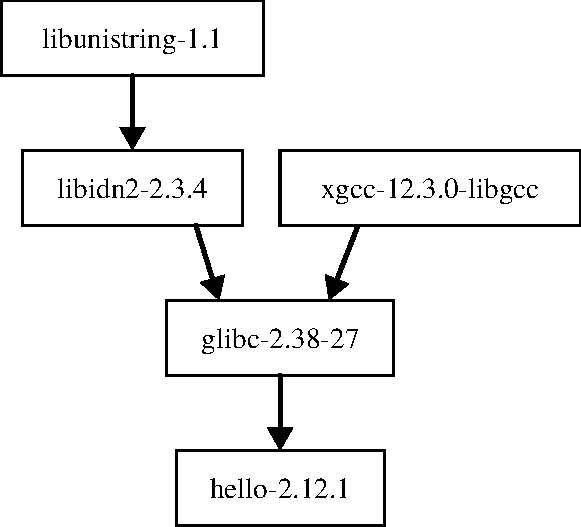
\includegraphics[width=0.5\linewidth]{./background/figures/nix/hello-pkg.pdf}
\end{figureBox}

For an example of making our own nix package. I have create a flake in Fig~ that builds the basic "hello" package also available on \texttt{nixpkgs}. \\

Highlighting particular lines in the \texttt{flake.nix} \\

\textbf{Line 2:} We have specified that we want to build our flake with the stable \textbf{nix channel} \texttt{nixos-23.11}, the most recent channel at the time of writing. This "channel" is really just a release branch on the nixpkgs github repository. Channels do receive conservative updates such as bug fixes and security patches but no major updates after initial release. The first time I build the hello package from my \texttt{flake.nix} a \texttt{flake.lock} is automatically generated that pins us to a specific revision of \texttt{nixos-23.11}. Our built inputs will not change until we relock our flake to either a different revision of \texttt{nixos-23.11} or a new channel entirely. \\

\textbf{Line 5:} Here we define \texttt{outputs} as a function that accepts, \texttt{self} (the flake) and \texttt{nixpkgs} (the set of packages we just pinned to on the line 2). What nix does is resolves all inputs and then calls the \texttt{output} function.\\

\textbf{Line 6:} Here we specify that we are defining the default package for users on \texttt{x86\_64-linux}. If we tried to build this package on a different cpu architecture like for example ARM (\texttt{aarch64-linux}) the flake would refuse to build the package  as it has not been defined for ARM yet. If we desired we could fix this by adding a \texttt{defaultPackage.aarch64-linux} definition.\\

\textbf{Line 7-9:} Here we are just defining a shorthand way to referring to x86 linux packages. This syntax is similar if not identical to Haskell.\\

\textbf{Line 10:} Here we begin the definition of the derivation which is the instruction set nix uses to build the package.\\

\textbf{Line 14:} We specify here that we need \texttt{gcc} in our sandbox to build our package. \texttt{gcc} here is shorthand for \texttt{gcc12} but we could specify and c compiler and version of that compiler we liked. If you really wanted to you could compile different parts of the code with different versions of gcc.\\

\textbf{Line 15:} Here we are slightly abusing the configure phase to generate a hello.c file. Each phase is essentially run as a bash script. Everything inside \texttt{mkDerivation} is happening inside a sandbox and will be discarded once the package is built (techically after we garbage collect). \\

\textbf{Line 16:} Here we actually build our package \\

\textbf{Line 17:} In this line we copy our executable we have generate which is currently in the sandbox into the actual package we are producing. \\
